
%(BEGIN_QUESTION)
% Copyright 2011, Tony R. Kuphaldt, released under the Creative Commons Attribution License (v 1.0)
% This means you may do almost anything with this work of mine, so long as you give me proper credit

In this process, a single ``shutdown controller'' device sends actuating signals to two solenoid trip valves, actuating them simultaneously:

$$\includegraphics[width=15.5cm]{i03857x01.eps}$$

One solenoid valve has an MTBF of 6.5 years, while the other has an MTBF of 4.1 years.

\vskip 10pt

Calculate the probability of this solenoid valve system failing to open the process line valve, assuming both valves are absolutely brand-new, and already burned-in by the manufacturer.

\vskip 10pt

Next, calculate the probability of this solenoid valve system failing to open the process line valve after 1 year of continuous operation.

\underbar{file i03857}
%(END_QUESTION)





%(BEGIN_ANSWER)

PFD (brand-new) = 0

\vskip 10pt

PFD (1 yr) = 0.328169

%(END_ANSWER)





%(BEGIN_NOTES)

At $t$ = 0, the reliability (R) for each solenoid is 100\%, and so there is no probability of failure on demand (PFD = 0).

\vskip 10pt

After 1 year, the reliability of each solenoid drops off accordingly:

$$R = e ^{- t \over MTBF}$$

$$R = e ^{- {1 \over 6.5}} = 0.857404$$

$$R = e ^{- {1 \over 4.1}} = 0.783564$$

This means the PFD for each solenoid (probability of {\it not} functioning as designed) will be 0.142596 and 0.216436, respectively.

\vskip 10pt

We can see from the diagram that both solenoids must successfully trip in order to open the process line valve.  Therefore, the PFD for the whole system is the probability that the first solenoid {\it or} the second solenoid will both fail.  This is equal to 0.328169.

%INDEX% Safety, system reliability: Mean Time Between Failures (MTBF)
%INDEX% Safety, system reliability: probability of failure on demand (PFD)

%(END_NOTES)


